%! Tex program = pdflatex
 
\documentclass[UTF8]{ctexart}
\CTEXsetup[format={\Large\bfseries}]{section}
\usepackage{amsmath}
\usepackage{ctex}
\usepackage{array}
\usepackage{ulem}
\usepackage{graphicx}
\usepackage{geometry}
\usepackage{multirow}
\usepackage{subfig}
\usepackage{float}
\usepackage{multicol}
\usepackage{multirow}
\usepackage{indentfirst}
\usepackage{makecell}
\geometry{papersize={21cm,29.7cm}}
\geometry{left=2.54cm,right=2.54cm,top=3.18cm,bottom=3.18cm}
\usepackage{fancyhdr}
\pagestyle{fancy}
\lhead{\today}
\chead{}
\rhead{2020011075}
\lfoot{清华大学}
\cfoot{\thepage}
\rfoot{物理实验B(1)}
\renewcommand{\headrulewidth}{0.4pt}
\renewcommand{\headwidth}{\textwidth}
\renewcommand{\footrulewidth}{0pt}
\usepackage{bm}
\begin{document}
\begin{titlepage}
    \begin{center}
		\quad \\
		\quad \\
        \quad \\
        \quad \\
        \quad \\
        \quad \\
		\kaishu \fontsize{30}{15} 阻尼振动和受迫振动实验报告

	\end{center}
	\vskip 10cm

    \begin{center}
        \begin{large}
        \begin{tabular}{cc}
        院\qquad 系:& ~~~~~~~~自动化系~~~~~~~~      \\
        \cline{2-2}\\
        班\qquad 级:& 自02班   \\
        \cline{2-2}\\
        学生姓名:& 彭程    \\
        \cline{2-2}\\
        学\qquad 号:&2020011075   \\
        \cline{2-2}\\
        组\qquad 号:& 单一晚M    \\
        \cline{2-2}\\
        座~~位~~号:& \# 13    \\
        \cline{2-2}
        \end{tabular}
        \end{large}
        \end{center}

\end{titlepage}
\newpage
\tableofcontents
\newpage
\section{实验名称}
直流电桥测电阻
\section{实验目的}
\begin{enumerate}
\item 观测阻尼振动,学习测量振动系统基本参数的方法。
\item 研究受迫振动的幅频特性和相频特性,观察共振现象。
\item 观测不同阻尼对受迫振动的影响。
\end{enumerate}
\section{实验原理}
    \subsection{阻尼振动运动方程} 



    对弹簧与撰轮的振动系统而言, 设转动惯量为  J , 转角  $\theta$ , 阻力矩
      $\gamma \frac{\mathrm{d} \theta}{\mathrm{d} t}$ , 弹簧力矩 $ -k \theta_{0} $ 令 $ \omega_{0}=\sqrt{k / J}$ , 阻尼系数 $ \beta=\gamma / 2 J$ , 可得摆轮运动方程为:
    $$
    \frac{\mathrm{d}^{2} \theta}{\mathrm{d} t^{2}}+2 \beta \frac{\mathrm{d} \theta}{\mathrm{d} t}+\omega_{0}^{2} \theta=0
    $$

    当  $\beta^{2}-\omega_{0}^{2}<0 $ 时, 解为
    $$
    \theta(t)=\theta_{i} \exp (-\beta t) \cos \left(\sqrt{\omega_{0}^{2}-\beta^{2} t}+\phi\right)
    $$

    周期
    $$
    T_{d}=\frac{2 \pi}{\sqrt{\omega_{0}^{2}-\beta^{2}}}
    $$

     \subsection{电机运动时的受迫振动运动方程} 
    电机通过连杆 $ \mathrm{E} $ 策动摆轮, 摇杆 $ M $ 转角 $ \alpha(t)=\frac{r}{R} \cos \omega t$  。令 $ \alpha_{m}=\frac{r}{R}$ , 得摆轮运动方程:
    $$
    J \frac{\mathrm{d}^{2} \theta}{\mathrm{d} t^{2}}+\gamma \frac{\mathrm{d} \theta}{\mathrm{d} t}+k \theta=k \alpha_{m} \cos \omega t
    $$

    同理, 可求得解为
    $$
    \theta_{\text {force }}=\theta_{\text {damp }}+\theta_{m} \cos \left(\omega t-\phi_{0}\right)
    $$

    其中:
    $$
    \theta_{m}=\frac{\alpha \omega_{0}^{2}}{\sqrt{\left(\omega_{0}^{2}-\omega^{2}\right)^{2}+4 \beta^{2} \omega^{2}}}, \phi_{0}=\arctan \left(\frac{2 \beta \omega}{\omega_{0}^{2}-\omega^{2}}\right)
    $$

    令阻尼比  $\zeta=\frac{\beta}{\omega_{0}}$ , 频率比 $ r=\frac{\omega}{\omega_{0}} $ 故幅频特性和相频特性分别为
    $$
    \theta_{m}=\frac{\alpha_{m}}{\sqrt{\left(1-r^{2}\right)^{2}+4 \zeta^{2} r^{2}}}, \phi=\arctan \left(\frac{2 \zeta r}{1-r^{2}}\right)
    $$

    \section{实验仪器}
    \noindent 波耳共振仪


    \section{实验任务}
    \subsection{实验步骤} 

    \noindent  (1) 调整仪器。打开电源开关,关断电机和闪光灯开关;阻尼开关置于“0”档;将有机玻璃转盘 F
    归零;拨动摆轮偏离平衡位置 $150\circ − 200\circ$,检查摆轮的自由摆动情况。\\
    
    \noindent  (2) 测量最小阻尼时(阻尼开关置于“0”档)的阻尼比 $\zeta $ 和固有角频率 $\omega_0$。阻尼开关置“摆轮”,选
    择最小阻尼周期选择置于“10”位置。拨动摆轮偏离平衡位置$ 150\circ − 200\circ$,读取显示窗中的振幅值。
    计时停止后,读取数据 $10Td$ 并立即按复位按钮启动周期测量。\\
    
    \noindent  (3) 仿照上述方法,测量其他阻尼状态的振幅。要求振动次数大于 10 次,需要测量每次振动的周期,
    周期选择置于“1”位置。\\
    
    \noindent  (4) 测定受迫振动的幅频特性和相频特性曲线。开启电机开关,开关置强迫力,周期选择置于“1”,
    调节旋钮改变电机转动频率 $\omega$,在稳定后读取振幅$ \theta_m$、周期$ T_d$、相位差 $\phi_0$。至少要有 12 个数据点,
    其中要包括共振点,即 $\phi = \pi /2$ 的点。\\
    
    \noindent  (5) 对数据进行分析处理,描绘曲线。

    \subsection{注意事项}

    \noindent 1.为避免剩磁影响,阻尼开关不要随便拨动;\\

    \noindent 2.只有测受迫振动相频特性时才开启仪器面板上的闪光灯开关,读完数据后迅即关闭;\\

    \noindent 3. 相频特性与幅频特性测量要在振动稳定后进行,可根据测量数据计算$ \omega$ 值和达到稳定态($e^{-t/\tau}<0.01$)
    所需要的时间;\\

    \noindent 4.在共振点附近要注意随时调节 勿使振幅过大($A_max<220\circ$)以免损坏波耳共振仪,在阻尼较小时尤
    其要小心操作。\\

    \noindent 5.几种阻尼状态下的幅频特性曲线和相频特性曲线要画在同一张坐标纸上,以便进行比较。




\section{数据处理}

\subsection{测量最小阻尼时的阻尼比  $\zeta$  和固有角频率  $\omega_{0}$}

\subsubsection{阻尼比 $ \zeta$  的计算}

测量最小阻尼时的振幅值 $ \theta_{j}$ , 共测得 50 个  $\theta_{j}$  的值。由于:
$$
\ln \theta_{j}-\ln \theta_{j-1}=-\beta T_{d}=-\beta \frac{2 \pi}{\sqrt{\omega_{0}^{2}-\beta^{2}}}=-\frac{2 \pi}{\sqrt{\zeta^{-2}-1}}
$$

根据上一表达式, 考虑对振幅 $ \theta_{j} $ 取对数, 则  $\ln \theta_{j}$  为等差级数 ,利用逐差法处理数据:
设  $I=\left[\frac{n}{2}\right]=25$ , 定义逐差值  $D_{j}=\ln \theta_{j+25}-\ln \theta_{j}(j=1, \cdots, 25) $, 计算结果如下表 。

\begin{center}
    \begin{tabular}{|c|c|c|c|c|c|c|c|}
        \hline   次数  i &  振幅  $\theta_{j} /^{\circ}$ & $\ln \theta_{j} $&  次数  i &  振幅  $\theta_{i} /^{\circ}$ & $\ln \theta_{i}$& 序号& $D_j=\ln \theta_{j+I}-\ln \theta_{j}$ \\
        \hline 1 & 168 & 5.124 & 26 & 141 & 4.949 &1     & -0.175  \\
        \hline 2 & 167 & 5.118 & 27 & 140 & 4.942 &2     & -0.176 \\
        \hline 3 & 166 & 5.112 & 28 & 139 & 4.934 &3     & -0.178 \\
        \hline 4 & 165 & 5.106 & 29 & 138 & 4.927 &4     & -0.179 \\
        \hline 5 & 163 & 5.094 & 30 & 137 & 4.920 &5     & -0.174 \\
        \hline 6 & 163 & 5.094 & 31 & 136 & 4.913 &6     & -0.181 \\
        \hline 7 & 161 & 5.081 & 32 & 135 & 4.905 &7     & -0.176 \\
        \hline 8 & 160 & 5.075 & 33 & 134 & 4.898 &8     & -0.177 \\
        \hline 9 & 159 & 5.069 & 34 & 133 & 4.890 &9     & -0.179 \\
        \hline 10 & 158 & 5.063 & 35 & 132 & 4.883 &10   & -0.180 \\
        \hline 11 & 157 & 5.056 & 36 & 131 & 4.875 &11   & -0.181 \\
        \hline 12 & 156 & 5.050 & 37 & 130 & 4.868 &12   & -0.182 \\
        \hline 13 & 155 & 5.043 & 38 & 129 & 4.860 &13   & -0.183 \\
        \hline 14 & 153 & 5.030 & 39 & 128 & 4.852 &14   & -0.178 \\
        \hline 15 & 153 & 5.030 & 40 & 127 & 4.844 &15   & -0.186\\
        \hline 16 & 151 & 5.017 & 41 & 126 & 4.836 &16   & -0.181\\
        \hline 17 & 150 & 5.011 & 42 & 125 & 4.828 &17   & -0.183 \\
        \hline 18 & 149 & 5.004 & 43 & 124 & 4.820 &18   & -0.184 \\
        \hline 19 & 148 & 4.997 & 44 & 123 & 4.812 &19   & -0.185\\
        \hline 20 & 147 & 4.990 & 45 & 122 & 4.804 &20   & -0.186 \\
        \hline 21 & 146 & 4.983 & 46 & 121 & 4.796 &21   & -0.187\\
        \hline 22 & 145 & 4.977 & 47 & 120 & 4.787 &22   & -0.190\\
        \hline 23 & 144 & 4.970 & 48 & 119 & 4.779 &23   & -0.191\\
        \hline 24 & 143 & 4.962 & 49 & 118 & 4.771 &24   & -0.191\\
        \hline 25 & 142 & 4.956 & 50 & 117 & 4.762 &25   & -0.194\\
        \hline
    \end{tabular}
\end{center}


\begin{align}
    \bar{D}&=\frac{1}{I} \sum_{j=1}^{I} D_{j}=\frac{-4.557}{25}=-0.182:  \nonumber  \\
    b&=\frac{1}{I^{2}} \sum_{j=1}^{I}\left(y_{j+I}-y_{j}\right)=\frac{-4.557}{25^{2}}=-0.00729 \nonumber \\
    S_{b}&=\frac{1}{I} \sqrt{\sum\left(D_{j}-\bar{D}\right)^{2} /(I-1)}=\frac{1}{25} \sqrt{7.09 \times 10^{-4} / 24}=2.174 \times 10^{-4} \nonumber 
\end{align}
    


而:
$$
b=-\frac{2 \pi}{\sqrt{\zeta^{2}-1}} 
$$

可得:
    $$
    \zeta=\sqrt{\frac{b^{2}}{4 \pi^{2}+b^{2}}}=\sqrt{\frac{{(-0.00729)}^{2}}{4 \pi^{2}+{(-0.00729)}^{2}}}=1.160 \times 10^{-3}
    $$


结合  $\zeta$  与  b  的关系式推导阻尼比的不确定度:

$$
\frac{\Delta_{\zeta}}{\zeta}=\sqrt{\left(\frac{\partial \ln \zeta}{\partial b} \Delta_{b}\right)^{2}}=\frac{4 \pi^{2}}{|b|\left(4 \pi^{2}+b^{2}\right)} \Delta_{b} \\
$$
$$
\Delta_{\zeta}=\zeta \frac{-4 \pi^{2}}{4 \pi^{2} b+b^{3}} \Delta_{b}=3.5 \times 10^{-5}
$$


将不确定度保留两位有效数字, 得  $\zeta $ 的最终结果为:
    $$
    \zeta=(1.160 \pm 0.035) \times 10^{-3}
    $$


    测得的连续 10 个周期的数据见下表 :

    \begin{center}
        \begin{tabular}{|c|c|c|c|c|c|}
            \hline 序号 & 1 & 2 & 3 & 4 & 5 \\
            \hline $T_{i}=10 \overline{T_{d}} / s$  &  15.052  &  15.062  &  15.054  &  15.047  &  15.049  \\
            \hline
        \end{tabular}
    \end{center}
  


    \subsubsection{周期计算}
    根据所测数据, 计算 $ \overline{T_{d}} $ 及不确定度 $ \Delta_{\overline{T_{d}}} $
    
    \begin{align}
    \overline{T_{d}}&=\frac{\sum_{i=1}^{5} T_{i}}{50}=1.5053 s \nonumber\\
    \Delta_{\overline{T_{d}}}&=\frac{T_{d}}{10^{5}}+0.001=1.015 \times 10^{-3} s\nonumber
    \end{align}
    
    周期的最终计算结果为:
    $$
    \overline{T_{d}}=(1.5053 \pm 0.0010) s
    $$
        
    \subsubsection{固有角频率计算}
    计算  $\omega_{0} $:
    $$
    \omega_{0}=\frac{2 \pi}{\overline{T_{d}} \sqrt{1-\zeta^{2}}}=\frac{2 \pi}{1.5053 \sqrt{1-\left(1.160 \times 10^{-3}\right)^{2}}}=4.1740 \mathrm{rad} / \mathrm{s}
    $$

    计算  $\omega_{0} $ 的不确定度:

    $$
    \frac{\Delta_{\omega_{0}}}{\omega_{0}}=\sqrt{\left(\frac{\partial \ln \omega_{0}}{\partial T_{d}} \Delta_{T_{d}}\right)^{2}+\left(\frac{\partial \ln \omega_{0}}{\partial \zeta} \Delta_{\zeta}\right)^{2}}
    $$

    由上式变换, 代入数据得:
    
    \begin{align}
    \Delta_{\omega_{0}}&=\omega_{0} \sqrt{\left(\frac{\Delta_{\overline{T_{d}}}}{\overline{T_{d}}}\right)^{2}+\left(\frac{\zeta \cdot \Delta_{\zeta}}{1-\zeta^{2}}\right)^{2}} \nonumber \\
    &=4.1740 \sqrt{\left(\frac{1.015 \times 10^{-3}}{1.5053}\right)^{2}+\left(\frac{1.160 \times 10^{-3} \times 3.5 \times 10^{-5}}{1-\left(1.160 \times 10^{-3}\right)^{2}}\right)^{2}} \nonumber\\
    &=2.814 \times 10^{-3} \mathrm{rad} / \mathrm{s} \nonumber
    \end{align}
    
    将不确定度保留两位有效数字, 固有角频率的最终计算结果为:
    $$
    \omega_{0}=(4.1740 \pm 0.0028) \mathrm{rad} / \mathrm{s}
    $$



\subsection{测量其余三种阻尼档位的阻尼比和固有角频率}

\subsubsection{阻尼档2}

测量数据如下:

\begin{tabular}{|c|c|c|c|c|c|c|c|c|}
    \hline   次数  i &  周期$T_d$&振幅  $\theta_{j} /^{\circ}$ & $\ln \theta_{j} $&  次数  i &周期$T_d$&  振幅  $\theta_{i} /^{\circ}$ & $\ln \theta_{i}$& 逐差值$D_j$ \\
    \hline 1 & 1.498 & 184 & 5.214936 & 7 & 1.504 & 109 & 4.691348 & -0.52359 \\
    \hline 2 & 1.499 & 169 & 5.129899 & 8 & 1.504 & 99 & 4.59512 & -0.53478 \\
    \hline 3 & 1.501 & 155 & 5.043425 & 9 & 1.505 & 91 & 4.51086 & -0.53257 \\
    \hline 4 & 1.501 & 142 & 4.955827 & 10 & 1.505 & 83 & 4.418841 & -0.53699 \\
    \hline 5 & 1.502 & 130 & 4.867534 & 11 & 1.505 & 75 & 4.317488 & -0.55005 \\
    \hline 6 & 1.503 & 119 & 4.779123 & 12 & 1.506 & 69 & 4.234107 & -0.54502 \\
    \hline
\end{tabular}\\

同理无阻尼情况的计算:
\begin{align}
    \bar{D}&=\frac{1}{I} \sum_{j=1}^{I} D_{j}=\frac{-3.223}{6}=-0.537:  \nonumber  \\
    b&=\frac{1}{I^{2}} \sum_{j=1}^{I}\left(y_{j+I}-y_{j}\right)=\frac{-3.223}{6^{2}}=-0.0895 \nonumber 
\end{align}
\begin{align}
    S_{b}&=\frac{1}{I} \sqrt{\sum\left(D_{j}-\bar{D}\right)^{2} /(I-1)}=\frac{1}{6} \sqrt{4.39 \times 10^{-4} /5}=1.562 \times 10^{-3} \nonumber \\
    \zeta&=\sqrt{\frac{b^{2}}{4 \pi^{2}+b^{2}}}=\sqrt{\frac{{(-0.0895)}^{2}}{4 \pi^{2}+{(-0.0895)}^{2}}}=1.424 \times 10^{-2}\nonumber\\
    \Delta_{\zeta}&=\zeta \frac{-4 \pi^{2}}{4 \pi^{2} b+b^{3}} \Delta_{b}=2.485 \times 10^{-4}\nonumber
\end{align}

将不确定度保留两位有效数字, 得  $\zeta $ 的最终结果为:
    $$
    \zeta=(1.424 \pm 0.025) \times 10^{-2}
    $$

计算 $ \overline{T_{d}} $ 及不确定度 $ \Delta_{\overline{T_{d}}} $

\begin{align}
\overline{T_{d}}&=\frac{\sum_{i=1}^{12} T_{i}}{12}=1.5028 s \nonumber\\
\Delta_{\overline{T_{d}}}&=\frac{T_{d}}{10^{5}}+0.001=1.015 \times 10^{-3} s\nonumber
\end{align}

周期的最终计算结果为:
$$
\overline{T_{d}}=(1.5028 \pm 0.0010) s
$$

计算  $\omega_{0} $:
$$
\omega_{0}=\frac{2 \pi}{\overline{T_{d}} \sqrt{1-\zeta^{2}}}=\frac{2 \pi}{1.5028 \sqrt{1-\left(1.42 \times 10^{-2}\right)^{2}}}=4.1814 \mathrm{rad} / \mathrm{s}
$$

计算  $\omega_{0} $ 的不确定度:

\begin{align}
\Delta_{\omega_{0}}&=\omega_{0} \sqrt{\left(\frac{\Delta_{\overline{T_{d}}}}{\overline{T_{d}}}\right)^{2}+\left(\frac{\zeta \cdot \Delta_{\zeta}}{1-\zeta^{2}}\right)^{2}} \nonumber \\
&=4.1814 \sqrt{\left(\frac{1.015 \times 10^{-3}}{1.5028}\right)^{2}+\left(\frac{1.424 \times 10^{-2} \times 2.5 \times 10^{-4}}{1-\left(1.424 \times 10^{-2}\right)^{2}}\right)^{2}} \nonumber\\
&=2.824 \times 10^{-3} \mathrm{rad} / \mathrm{s} \nonumber
\end{align}

将不确定度保留两位有效数字, 固有角频率的最终计算结果为:
$$
\omega_{0}=(4.1814 \pm 0.0028) \mathrm{rad} / \mathrm{s}
$$

计算阻尼系数$\beta$:
$$
\beta=\frac{1}{\tau}=\frac{b}{-T_{d}}=0.0596 \mathrm{rad} / \mathrm{s}
$$

可以得到:
$$
\tau=\frac{1}{\zeta \omega}=16.79 s, \quad \frac{\Delta_{\tau}}{\tau}=\sqrt{\left(\frac{\Delta_{\zeta}}{\zeta}\right)^{2}+\left(\frac{\Delta_{\omega_{0}}}{\omega_{0}}\right)^{2}}=0.017, \quad \Delta_{\tau}=0.29
$$

所以得到:
$$
\tau=16.79 \pm 0.29 s
$$

同时有:
$$
Q=\frac{1}{2 \zeta}=35.11, \frac{\Delta_{Q}}{Q}=\sqrt{\left(\frac{\Delta_{\zeta}}{\zeta}\right)^{2}}=0.017, \Delta_{Q}=0.61
$$

所以得到:
$$
Q=35.11 \pm 0.61
$$



\subsubsection{阻尼档3}
测量数据如下:

\begin{tabular}{|c|c|c|c|c|c|c|c|c|}
\hline   次数  i &  周期$T_d$&振幅  $\theta_{j} /^{\circ}$ & $\ln \theta_{j} $&  次数  i &周期$T_d$&  振幅  $\theta_{i} /^{\circ}$ & $\ln \theta_{i}$& 逐差值$D_j$ \\
\hline 1 & 1.496 & 191 & 5.252273 & 7 & 1.504 & 97 & 4.574711 & -0.67756 \\
\hline 2 & 1.499 & 171 & 5.141664 & 8 & 1.505 & 87 & 4.465908 & -0.67576 \\
\hline 3 & 1.501 & 153 & 5.030438 & 9 & 1.505 & 77 & 4.343805 & -0.68663 \\
\hline 4 & 1.501 & 137 & 4.919981 & 10 & 1.505 & 69 & 4.234107 & -0.68587 \\
\hline 5 & 1.502 & 122 & 4.804021 & 11 & 1.506 & 61 & 4.110874 & -0.69315 \\
\hline 6 & 1.504 & 109 & 4.691348 & 12 & 1.506 & 54 & 3.988984 & -0.70236 \\
\hline
\end{tabular}

同理无阻尼情况的计算:
\begin{align}
    \bar{D}&=\frac{1}{I} \sum_{j=1}^{I} D_{j}=\frac{-4.121}{6}=-0.687:  \nonumber  \\
    b&=\frac{1}{I^{2}} \sum_{j=1}^{I}\left(y_{j+I}-y_{j}\right)=\frac{-4.121}{6^{2}}=-0.114 \nonumber \\
    S_{b}&=\frac{1}{I} \sqrt{\sum\left(D_{j}-\bar{D}\right)^{2} /(I-1)}=\frac{1}{6} \sqrt{4.91\times 10^{-4} /5}=1.652 \times 10^{-3} \nonumber \\
    \zeta&=\sqrt{\frac{b^{2}}{4 \pi^{2}+b^{2}}}=\sqrt{\frac{{(-0.114)}^{2}}{4 \pi^{2}+{(-0.114)}^{2}}}=1.814 \times 10^{-2}\nonumber\\
    \Delta_{\zeta}&=\zeta \frac{-4 \pi^{2}}{4 \pi^{2} b+b^{3}} \Delta_{b}=2.627 \times 10^{-4}\nonumber
\end{align}

将不确定度保留两位有效数字, 得  $\zeta $ 的最终结果为:
    $$
    \zeta=(1.814 \pm 0.027) \times 10^{-2}
    $$

计算 $ \overline{T_{d}} $ 及不确定度 $ \Delta_{\overline{T_{d}}} $

\begin{align}
\overline{T_{d}}&=\frac{\sum_{i=1}^{12} T_{i}}{12}=1.5028 s \nonumber\\
\Delta_{\overline{T_{d}}}&=\frac{T_{d}}{10^{5}}+0.001=1.015 \times 10^{-3} s\nonumber
\end{align}

周期的最终计算结果为:
$$
\overline{T_{d}}=(1.5028 \pm 0.0010) s
$$

计算  $\omega_{0} $:
$$
\omega_{0}=\frac{2 \pi}{\overline{T_{d}} \sqrt{1-\zeta^{2}}}=\frac{2 \pi}{1.5028 \sqrt{1-\left(1.814 \times 10^{-2}\right)^{2}}}=4.1817 \mathrm{rad} / \mathrm{s}
$$

计算  $\omega_{0} $ 的不确定度:

\begin{align}
\Delta_{\omega_{0}}&=\omega_{0} \sqrt{\left(\frac{\Delta_{\overline{T_{d}}}}{\overline{T_{d}}}\right)^{2}+\left(\frac{\zeta \cdot \Delta_{\zeta}}{1-\zeta^{2}}\right)^{2}} \nonumber \\
&=4.1817 \sqrt{\left(\frac{1.015 \times 10^{-3}}{1.5028}\right)^{2}+\left(\frac{1.814 \times 10^{-2} \times 2.7 \times 10^{-4}}{1-\left(1.814 \times 10^{-2}\right)^{2}}\right)^{2}} \nonumber\\
&=2.824 \times 10^{-3} \mathrm{rad} / \mathrm{s} \nonumber
\end{align}

将不确定度保留两位有效数字, 固有角频率的最终计算结果为:
$$
\omega_{0}=(4.1817 \pm 0.0028) \mathrm{rad} / \mathrm{s}
$$

计算阻尼系数$\beta$:
$$
\beta=\frac{1}{\tau}=\frac{b}{-T_{d}}=0.0759 \mathrm{rad} / \mathrm{s}
$$

可以得到:
$$
\tau=\frac{1}{\zeta \omega}=13.18 s, \quad \frac{\Delta_{\tau}}{\tau}=\sqrt{\left(\frac{\Delta_{\zeta}}{\zeta}\right)^{2}+\left(\frac{\Delta_{\omega_{0}}}{\omega_{0}}\right)^{2}}=0.014, \quad \Delta_{\tau}=0.18
$$

所以得到:
$$
\tau=13.18 \pm 0.18 s
$$

同时有:
$$
Q=\frac{1}{2 \zeta}=27.56, \frac{\Delta_{Q}}{Q}=\sqrt{\left(\frac{\Delta_{\zeta}}{\zeta}\right)^{2}}=0.014, \Delta_{Q}=0.40
$$

所以得到:
$$
Q=27.56 \pm 0.40
$$


\subsubsection{阻尼档4}

测量数据如下:

\begin{tabular}{|c|c|c|c|c|c|c|c|c|}
    \hline   次数  i &  周期$T_d$&振幅  $\theta_{j} /^{\circ}$ & $\ln \theta_{j} $&  次数  i &周期$T_d$&  振幅  $\theta_{i} /^{\circ}$ & $\ln \theta_{i}$& 逐差值$D_j$ \\
    \hline 1 & 1.501 & 174 & 5.159055 & 7 & 1.51 & 73 & 4.290459 & -0.8686 \\
    \hline 2 & 1.503 & 151 & 5.01728 & 8 & 1.509 & 63 & 4.143135 & -0.87415 \\
    \hline 3 & 1.505 & 131 & 4.875197 & 9 & 1.509 & 55 & 4.007333 & -0.86786 \\
    \hline 4 & 1.506 & 113 & 4.727388 & 10 & 1.51 & 47 & 3.850148 & -0.87724 \\
    \hline 5 & 1.508 & 98 & 4.584967 & 11 & 1.51 & 40 & 3.688879 & -0.89609 \\
    \hline 6 & 1.508 & 85 & 4.442651 & 12 & 1.511 & 35 & 3.555348 & -0.8873 \\
    \hline
\end{tabular}

同理无阻尼情况的计算:
\begin{align}
    \bar{D}&=\frac{1}{I} \sum_{j=1}^{I} D_{j}=\frac{-5.271}{6}=-0.879:  \nonumber  \\
    b&=\frac{1}{I^{2}} \sum_{j=1}^{I}\left(y_{j+I}-y_{j}\right)=\frac{-5.271}{6^{2}}=-0.146 \nonumber \\
    S_{b}&=\frac{1}{I} \sqrt{\sum\left(D_{j}-\bar{D}\right)^{2} /(I-1)}=\frac{1}{6} \sqrt{6.2\times 10^{-4} /5}=1.856 \times 10^{-3} \nonumber \\
    \zeta&=\sqrt{\frac{b^{2}}{4 \pi^{2}+b^{2}}}=\sqrt{\frac{{(-0.146)}^{2}}{4 \pi^{2}+{(-0.146)}^{2}}}=2.323 \times 10^{-2}\nonumber\\
    \Delta_{\zeta}&=\zeta \frac{-4 \pi^{2}}{4 \pi^{2} b+b^{3}} \Delta_{b}=2.951 \times 10^{-4}\nonumber
\end{align}

将不确定度保留两位有效数字, 得  $\zeta $ 的最终结果为:
    $$
    \zeta=(2.323 \pm 0.030) \times 10^{-2}
    $$

计算 $ \overline{T_{d}} $ 及不确定度 $ \Delta_{\overline{T_{d}}} $

\begin{align}
\overline{T_{d}}&=\frac{\sum_{i=1}^{12} T_{i}}{12}=1.5075 s \nonumber\\
\Delta_{\overline{T_{d}}}&=\frac{T_{d}}{10^{5}}+0.001=1.015 \times 10^{-3} s\nonumber
\end{align}

周期的最终计算结果为:
$$
\overline{T_{d}}=(1.5075 \pm 0.0010) s
$$

计算  $\omega_{0} $:
$$
\omega_{0}=\frac{2 \pi}{\overline{T_{d}} \sqrt{1-\zeta^{2}}}=\frac{2 \pi}{1.5075 \sqrt{1-\left(2.323 \times 10^{-2}\right)^{2}}}=4.1691 \mathrm{rad} / \mathrm{s}
$$

计算  $\omega_{0} $ 的不确定度:

\begin{align}
\Delta_{\omega_{0}}&=\omega_{0} \sqrt{\left(\frac{\Delta_{\overline{T_{d}}}}{\overline{T_{d}}}\right)^{2}+\left(\frac{\zeta \cdot \Delta_{\zeta}}{1-\zeta^{2}}\right)^{2}} \nonumber \\
&=4.1691 \sqrt{\left(\frac{1.015 \times 10^{-3}}{1.5075}\right)^{2}+\left(\frac{2.323 \times 10^{-2} \times 2.9 \times 10^{-5}}{1-\left(2.323 \times 10^{-2}\right)^{2}}\right)^{2}} \nonumber\\
&=2.807 \times 10^{-3} \mathrm{rad} / \mathrm{s} \nonumber
\end{align}

将不确定度保留两位有效数字, 固有角频率的最终计算结果为:
$$
\omega_{0}=(4.1691 \pm 0.0028) \mathrm{rad} / \mathrm{s}
$$

计算阻尼系数$\beta$:
$$
\beta=\frac{1}{\tau}=\frac{b}{-T_{d}}=0.0968 \mathrm{rad} / \mathrm{s}
$$

可以得到:
$$
\tau=\frac{1}{\zeta \omega}=10.33 s, \quad \frac{\Delta_{\tau}}{\tau}=\sqrt{\left(\frac{\Delta_{\zeta}}{\zeta}\right)^{2}+\left(\frac{\Delta_{\omega_{0}}}{\omega_{0}}\right)^{2}}=0.013, \quad \Delta_{\tau}=0.13
$$

所以得到:
$$
\tau=10.33 \pm 0.13 s
$$

同时有:
$$
Q=\frac{1}{2 \zeta}=21.52, \frac{\Delta_{Q}}{Q}=\sqrt{\left(\frac{\Delta_{\zeta}}{\zeta}\right)^{2}}=0.013, \Delta_{Q}=0.28
$$

所以得到:
$$
Q=21.52 \pm 0.28
$$

\subsubsection{参数汇总}

\begin{tabular}{|c|c|c|c|c|}
    \hline 阻尼状态  &  阻尼比  $\zeta$ &  周期 $T_{d} / s$ & $ 固有角频率 \omega_{0} / \mathrm{rad} \cdot \mathrm{s}^{-1}$ & $ 阻尼系数  \beta / \mathrm{rad} \cdot \mathrm{s}^{-1}$ \\
    \hline 2 & $(1.424 \pm 0.025) \times 10^{-2}$ & $1.5028 \pm 0.0010$&$ 4.1814 \pm 0.0028$ & 0.0596 \\
    \hline 3 & $(1.814 \pm 0.027) \times 10^{-2}$ & $1.5028 \pm 0.0010$& $4.1817 \pm 0.0028$ & 0.0759 \\
    \hline 4 & $(2.323 \pm 0.030) \times 10^{-2}$ & $1.5075 \pm 0.0010$& $4.1691 \pm 0.0028$ & 0.0968 \\
    \hline
    \end{tabular}

\subsection{测定受迫振动的幅频特性和相频特性曲线}

根据测得数据以及系统参数计算理论相位差 
 $\phi=\arctan \left(\frac{2 \beta \omega}{\omega_{0}^{2}-\omega^{2}}\right)$  、
 相位差的相对偏差  $\frac{\phi_{0}-\phi}{\phi}$  、测得的 $ \omega$  与理论值 $ \omega_{0}  $
 的比较 $ \frac{\omega}{\omega_{0}} $ 。

阻尼2时测量数据和计算结果:\\

\begin{tabular}{|c|c|c|c|c|c|c|c|c|c|}
    \hline 次数i &    $\theta_{i} /{ }^{\circ}$ & $T_{d} / \mathrm{s}$ & $\omega / \mathrm{rad} \cdot \mathrm{s}^{-1} $&$ \omega / \omega_{0}$ & $\phi_{1} /{ }^{\circ} $& $\phi_{2} /{ }^{\circ}$ & $\phi_{0} /{ }^{\circ} $&  理论值 $ \phi /{ }^{\circ}$ & $\frac{\phi_{0}-\phi}{\phi} /{ }^{\circ}$ \\
    \hline 1 & 36 & 1.602 & 3.922 & 0.938 & 10.0 & 14.5 & 12.3 & 12.5 & -2.00 \% \\
    \hline 2 & 46 & 1.577 & 3.984 & 0.953 & 14.0 & 18.5 & 16.3 & 16.4 & -0.91 \% \\
    \hline 3 & 54 & 1.565 & 4.015 & 0.960 & 17.0 & 21.0 & 19.0 & 19.3 & -1.55 \% \\
    \hline 4 & 70 & 1.547 & 4.062 & 0.971 & 26.0 & 29.0 & 27.5 & 26.1 & 5.36 \% \\
    \hline 5 & 91 & 1.534 & 4.096 & 0.980 & 36.0 & 38.0 & 37.0 & 34.6 & 6.94 \% \\
    \hline 6 & 135 & 1.511 & 4.158 & 0.994 & 72.0 & 74.0 & 73.0 & 68.8 & 6.10 \% \\
    \hline 7 & 144 & 1.505 & 4.175 & 0.998 & 79.0 & 81.0 & 80.0 & 83.7 & -4.42 \% \\
    \hline 8 & 150 & 1.501 & 4.186 & 1.001 & 91.0 & 93.0 & 92.0 & 85.6 & 7.48 \% \\
    \hline 9 & 143 & 1.497 & 4.197 & 1.004 & 105.5 & 107.0 & 106.3 & 104.8 & 1.38 \% \\
    \hline 10 & 133 & 1.493 & 4.208 & 1.006 & 115.5 & 117.5 & 116.5 & 114.3 & 1.92 \% \\
    \hline 11 & 120 & 1.490 & 4.217 & 1.008 & 123.0 & 125.0 & 124.0 & 120.7 & 2.73 \% \\
    \hline 12 & 97 & 1.484 & 4.234 & 1.013 & 134.0 & 136.0 & 135.0 & 131.2 & 2.90 \% \\
    \hline 13 & 71 & 1.473 & 4.266 & 1.020 & 141.5 & 144.0 & 142.8 & 144.4 & -1.14 \% \\
    \hline 14 & 52 & 1.458 & 4.309 & 1.031 & 154.0 & 157.0 & 155.5 & 154.7 & 0.52 \% \\
    \hline
\end{tabular}

阻尼3时测量数据和计算结果:\\

\begin{tabular}{|c|c|c|c|c|c|c|c|c|c|}
    \hline 次数i &    $\theta_{i} /{ }^{\circ}$ & $T_{d} / \mathrm{s}$ & $\omega / \mathrm{rad} \cdot \mathrm{s}^{-1} $&$ \omega / \omega_{0}$ & $\phi_{1} /{ }^{\circ} $& $\phi_{2} /{ }^{\circ}$ & $\phi_{0} /{ }^{\circ} $&  理论值 $ \phi /{ }^{\circ}$ & $\frac{\phi_{0}-\phi}{\phi} /{ }^{\circ}$ \\
    \hline 1 & 36 & 1.594 & 3.942 & 0.943 & 14.0 & 19.0 & 16.5 & 17.1 & -3.32 \% \\
    \hline 2 & 42 & 1.584 & 3.967 & 0.949 & 16.0 & 20.0 & 18.0 & 19.0 & -5.09 \% \\
    \hline 3 & 45 & 1.577 & 3.984 & 0.953 & 18.0 & 21.0 & 19.5 & 20.6 & -5.17 \% \\
    \hline 4 & 50 & 1.564 & 4.017 & 0.961 & 24.0 & 27.0 & 25.5 & 24.4 & 4.71 \% \\
    \hline 5 & 61 & 1.550 & 4.054 & 0.969 & 30.0 & 33.0 & 31.5 & 30.3 & 4.07 \% \\
    \hline 6 & 76 & 1.536 & 4.091 & 0.978 & 41.0 & 44.0 & 42.5 & 39.5 & 7.62 \% \\
    \hline 7 & 99 & 1.521 & 4.131 & 0.988 & 58.5 & 61.0 & 59.8 & 56.1 & 6.56 \% \\
    \hline 8 & 113 & 1.512 & 4.156 & 0.994 & 70.5 & 73.0 & 71.8 & 70.9 & 1.15 \% \\
    \hline 9 & 118 & 1.504 & 4.178 & 0.999 & 87.0 & 89.5 & 88.3 & 86.9 & 1.50 \% \\
    \hline 10 & 113 & 1.500 & 4.189 & 1.002 & 97.0 & 99.0 & 98.0 & 95.3 & 2.80 \% \\
    \hline 11 & 104 & 1.493 & 4.208 & 1.006 & 112.5 & 114.5 & 113.5 & 109.3 & 3.80 \% \\
    \hline 12 & 67 & 1.474 & 4.263 & 1.019 & 139.0 & 141.0 & 140.0 & 136.6 & 2.50 \% \\
    \hline 13 & 54 & 1.464 & 4.292 & 1.026 & 146.5 & 150.0 & 148.3 & 145.1 & 2.19 \% \\
    \hline 14 & 51 & 1.455 & 4.318 & 1.033 & 151.0 & 154.0 & 152.5 & 150.6 & 1.29 \% \\
    \hline
\end{tabular}\\

阻尼4时测量数据和计算结果:\\

\begin{tabular}{|c|c|c|c|c|c|c|c|c|c|}
    \hline 次数i &    $\theta_{i} /{ }^{\circ}$ & $T_{d} / \mathrm{s}$ & $\omega / \mathrm{rad} \cdot \mathrm{s}^{-1} $&$ \omega / \omega_{0}$ & $\phi_{1} /{ }^{\circ} $& $\phi_{2} /{ }^{\circ}$ & $\phi_{0} /{ }^{\circ} $&  理论值 $ \phi /{ }^{\circ}$ & $\frac{\phi_{0}-\phi}{\phi} /{ }^{\circ}$ \\
    \hline 1 & 43 & 1.577 & 3.984 & 0.956 & 23.5 & 27.5 & 25.5 & 27.1 & -5.92 \% \\
    \hline 2 & 48 & 1.566 & 4.012 & 0.962 & 29.0 & 32.0 & 30.5 & 31.2 & -2.20 \% \\
    \hline 3 & 54 & 1.552 & 4.048 & 0.971 & 36.0 & 40.0 & 38.0 & 38.3 & -0.85 \% \\
    \hline 4 & 64 & 1.544 & 4.069 & 0.976 & 43.0 & 46.0 & 44.5 & 43.8 & 1.57 \% \\
    \hline 5 & 69 & 1.533 & 4.099 & 0.983 & 53.0 & 56.0 & 54.5 & 53.7 & 1.47 \% \\
    \hline 6 & 77 & 1.522 & 4.128 & 0.990 & 65.0 & 67.0 & 66.0 & 67.0 & -1.51 \% \\
    \hline 7 & 81 & 1.515 & 4.147 & 0.995 & 74.0 & 77.0 & 75.5 & 77.3 & -2.31 \% \\
    \hline 8 & 83 & 1.508 & 4.167 & 0.999 & 84.0 & 86.5 & 85.3 & 88.5 & -3.67 \% \\
    \hline 9 & 87 & 1.504 & 4.178 & 1.002 & 92.0 & 94.0 & 93.0 & 95.0 & -2.15 \% \\
    \hline 10 & 85 & 1.498 & 4.194 & 1.006 & 100.0 & 103.0 & 101.5 & 104.6 & -2.96 \% \\
    \hline 11 & 77 & 1.489 & 4.220 & 1.012 & 114.0 & 117.0 & 115.5 & 117.5 & -1.68 \% \\
    \hline 12 & 65 & 1.476 & 4.257 & 1.021 & 129.0 & 133.0 & 131.0 & 131.9 & -0.69 \% \\
    \hline 13 & 55 & 1.465 & 4.289 & 1.029 & 138.0 & 141.0 & 139.5 & 140.7 & -0.82 \% \\
    \hline 14 & 44 & 1.451 & 4.330 & 1.039 & 146.0 & 148.5 & 147.3 & 148.5 & -0.86 \% \\
    \hline
\end{tabular}\\


绘制幅频、相频特性曲线如下:


\begin{figure}[H]
    \centering
    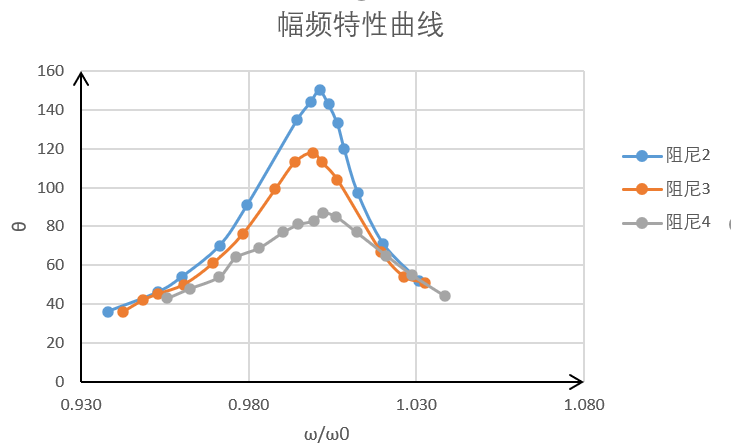
\includegraphics[scale=1]{幅频特性曲线.png}
    \caption{幅频特性曲线}
    \label{fig:label}
\end{figure}


\begin{figure}[H]
    \centering
    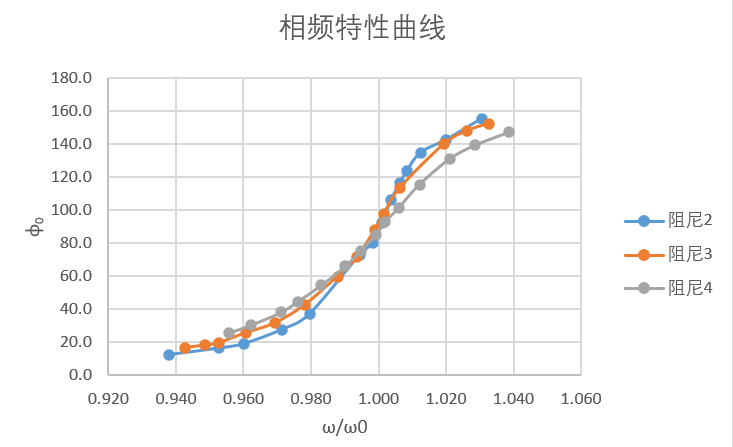
\includegraphics[scale=1]{相频特性曲线.png}
    \caption{相频特性曲线}
    \label{fig:label}
\end{figure}

根据测得的共振点  $\left(\phi=90^{\circ}\right)$  的数据, 可得测得的  $\omega $ 值分别为: $ \omega_{2}=4.183 $、 $\omega_{3}=4.178$ 、 $\omega_{4}=4.175 $
与固有角频率的相对误差分别为:$\Delta E_{2}=0.04 \% 、 \Delta E_{3}=0.09 \% 、 \Delta E_{4}=0.14 \%$。

相位差$\phi$的相对偏差见表格最后一栏。

\section{实验小结}

\subsection{思考题}

\noindent  \textbf{(1)如何判断受迫振动已处于稳定状态?}

可利用时间常数 $\tau$。经过$ 3 \sim 5\tau$ 后,随时间衰减的指数下降到初值的 $e^{−5} \sim e^{−3}$,可以认为趋于稳定。

实际测量中,可以通过观察振幅来判断。 当仪表上振幅的测量值保持在某个数值不变时, 受迫振动已
经处于稳定状态。实际操作中,当
20 个周期左右系统的振幅不再改变时,即可认为达到平衡态。



\noindent  \textbf{(2)从幅频曲线的相对振幅比为 1/2 的点,也可求出$\beta$ 值。试用你作出的幅频特性曲线进行计算,把结
果与练习 2 的结果相比较。}

共振时, 有:

\begin{align}
\omega &=\sqrt{\omega_{0}^{2}-2 \beta^{2}} \nonumber\\
\theta_{m} &=\frac{\alpha_{m} \omega_{0}^{2}}{2 \beta \sqrt{\omega_{0}^{2}-\beta^{2}}} \nonumber
\end{align}

因此, 任意振幅下:

$$
\frac{\theta}{\theta_{m}}=\frac{2 \beta \sqrt{\omega_{0}^{2}-\beta^{2}}}{\sqrt{\left(\omega_{0}^{2}-\omega_{2}\right)^{2}+4 \beta^{2} \omega^{2}}} \approx \frac{\beta}{\sqrt{\left(\omega_{0}-\omega\right)^{2}+\beta^{2}}}
$$

令 $ \frac{\theta}{\theta_{m}}=\frac{1}{2} $

$$
\beta=\frac{\left|\omega-\omega_{0}\right|}{\sqrt{3}}
$$

作振幅等于一半最大振幅的水平线, 与曲线交于两点, 计算两点横坐标与固有频率差的绝对值, 取平均后代入公式即可计算阻尼系数 $ \beta$  。

对阻尼 2, $\theta=75^{\circ}$ , 读图得交点分别为  $\omega_{1} / \omega_{0}=0.973$ 、$ \omega_{2} / \omega_{0}=1.018 $ 。
$$
\beta=\frac{\left|\omega-\omega_{0}\right|}{\sqrt{3}}=\frac{0.5 \times 4.1814(|0.973-1|+|1.018-1|)}{\sqrt{3}}=0.0563 \mathrm{rad} / \mathrm{s}
$$

相对误差为  5.53 \% 

对阻尼  3, $\theta=59^{\circ}$ , 读图得交点分别为 $ \omega_{1} / \omega_{0}=0.968$ 、$ \omega_{2} / \omega_{0}=1.024 $ 。
$$
\beta=\frac{\left|\omega-\omega_{0}\right|}{\sqrt{3}}=\frac{0.5 \times 4.1817(|0.968-1|+|1.024-1|)}{\sqrt{3}}=0.0736 \mathrm{rad} / \mathrm{s}
$$

相对误差为  3.03 \% 

对阻尼  4, $\theta=44^{\circ}$ , 读图得交点分别为 $ \omega_{1} / \omega_{0}=0.957$ 、$ \omega_{2} / \omega_{0}=1.039 $ 。
$$
\beta=\frac{\left|\omega-\omega_{0}\right|}{\sqrt{3}}=\frac{0.5 \times 4.1691(|0.957-1|+|1.039-1|)}{\sqrt{3}}=0.0987 \mathrm{rad} / \mathrm{s}
$$

相对误差为  1.96 \% 

\noindent  \textbf{(3) 实验中如何判断达到共振?共振频率是多少?}

由相频特性曲线与幅频特性曲线:

\begin{align}
\phi(r)&=\arctan \left(\frac{2 \zeta r}{1-r^{2}}\right) \nonumber\\
\theta_{m}(r)&=\frac{\alpha_{m}}{\sqrt{\left(1-r^{2}\right)^{2}+4 \zeta^{2} r^{2}}}\nonumber
\end{align}


实验测得的共振频率分别为: $ \omega_{2}=4.181 \mathrm{rad} / \mathrm{s} $、 $\omega_{3}=4.181 \mathrm{rad} / \mathrm{s}$ 、 $\omega_{4}=4.169 \mathrm{rad} / \mathrm{s} $

实验中通过调节强制力的周期来达到共振, 调节过程中, 一是可以看振幅的变化, 振幅 最大时达到共振; 二是可以看相位差  $\phi $ 的变化, 达到$90^\circ$ 的时候达到共振。
除此之外, 还可以绘制幅频特性曲线, 曲线中最高点发生共振, 其对应的频率就是共振频率。

共振频率的计算:
$ \omega=\sqrt{\omega_{0}{ }^{2}-(2 \beta)^{2}} $,~~~$f=\frac{2\pi}{\omega}$。


\subsection{总结}

通过本次观测阻尼振动和受迫振动的实验,我更好地理解阻尼振动与受迫振动,成功测量了阻尼振动和受迫振动的参数, 画出受迫振动幅频特性曲线和相频特性曲线。

同时,根据实验结果所反映出的误差,我也仔细分析和反思了实验中一些可能引起误差的地方,如:
测量十倍周期时可能因为复位不及时造成误差;
 测量受迫振动时, 需要等待振动稳定下来再读数, 虽然已等待一段时间, 但仍可能
振动实际上并未稳定, 带来误差;
 仪器误差, 如光电门安装位置不准等, 可能带来误差, 这个也是本实验误差的重要
原因。

总体来说,本实验整体进行的比较顺利, 但是因为在实验过程中需要等待振动稳定等原因, 实验整体持续了很长时间。



最后感谢助教的悉心指导!
\\
\\

\section{预习思考题}
\begin{figure}[H]
    \centering
    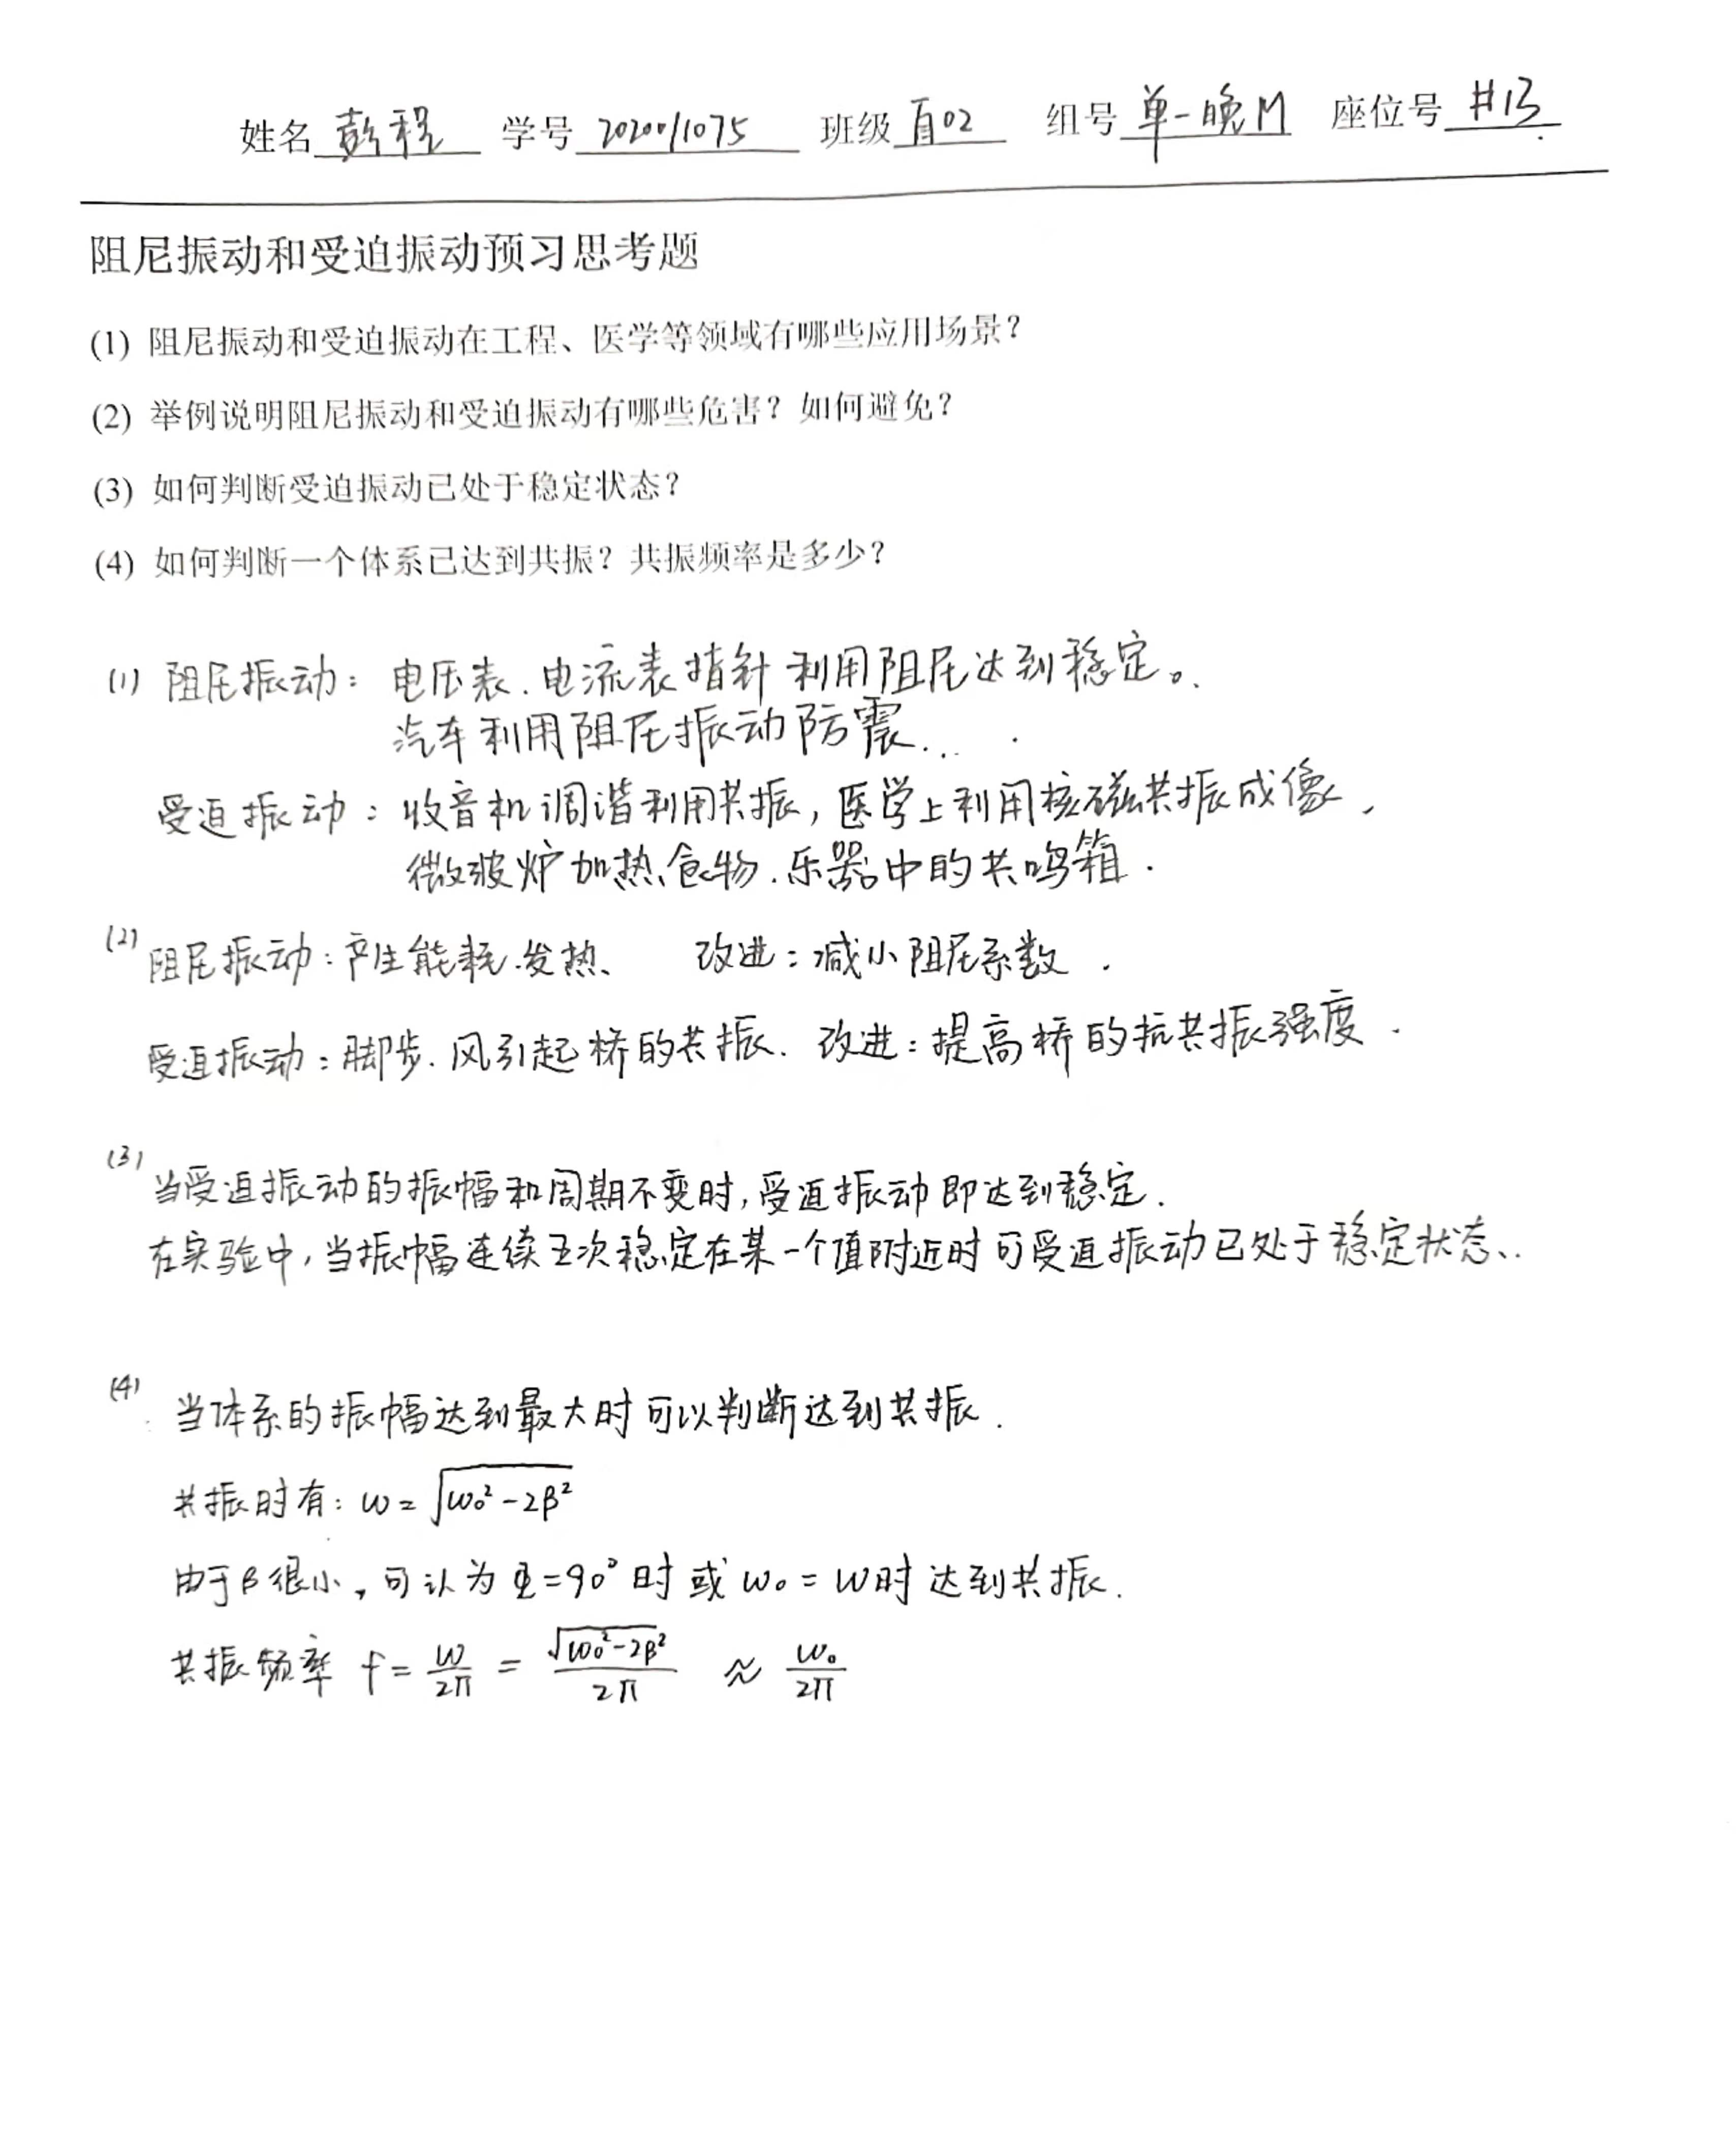
\includegraphics[scale=0.13]{预习思考题.jpg}
\end{figure}


\section{原始数据记录}
\begin{figure}[H]
    \centering
    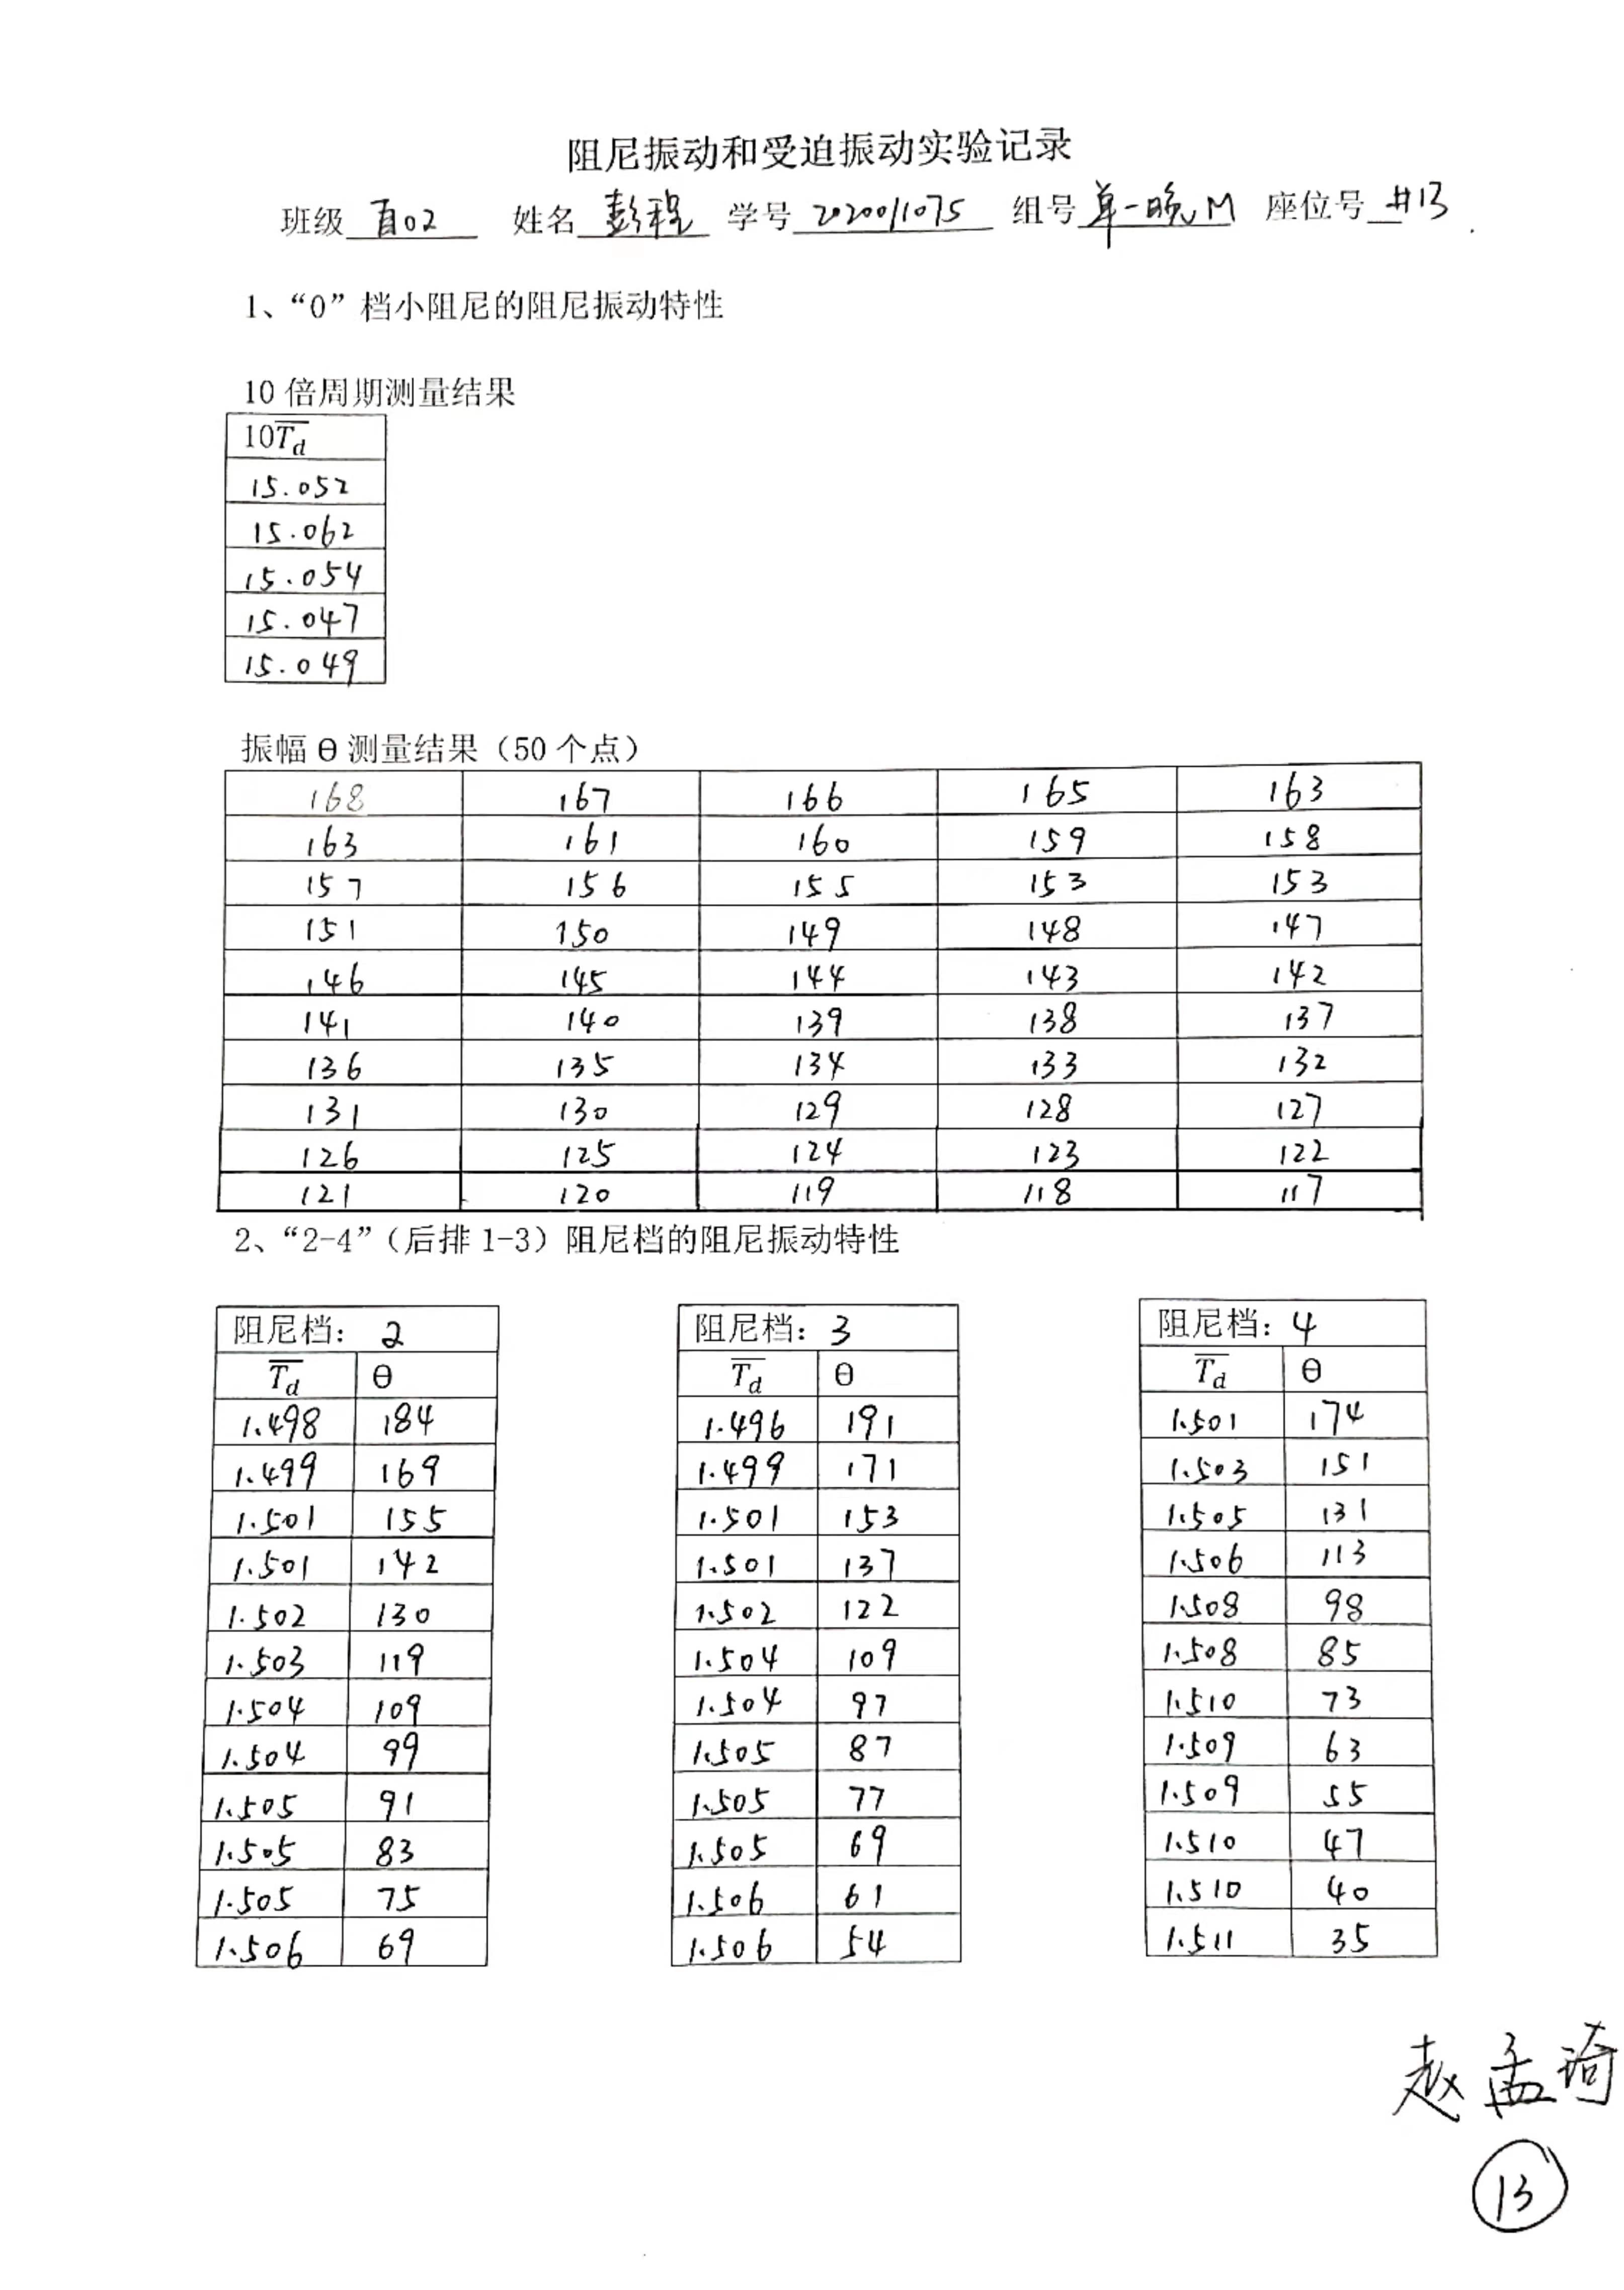
\includegraphics[scale=0.14]{原始数据1.jpg}
\end{figure}
\begin{figure}[H]
    \centering
    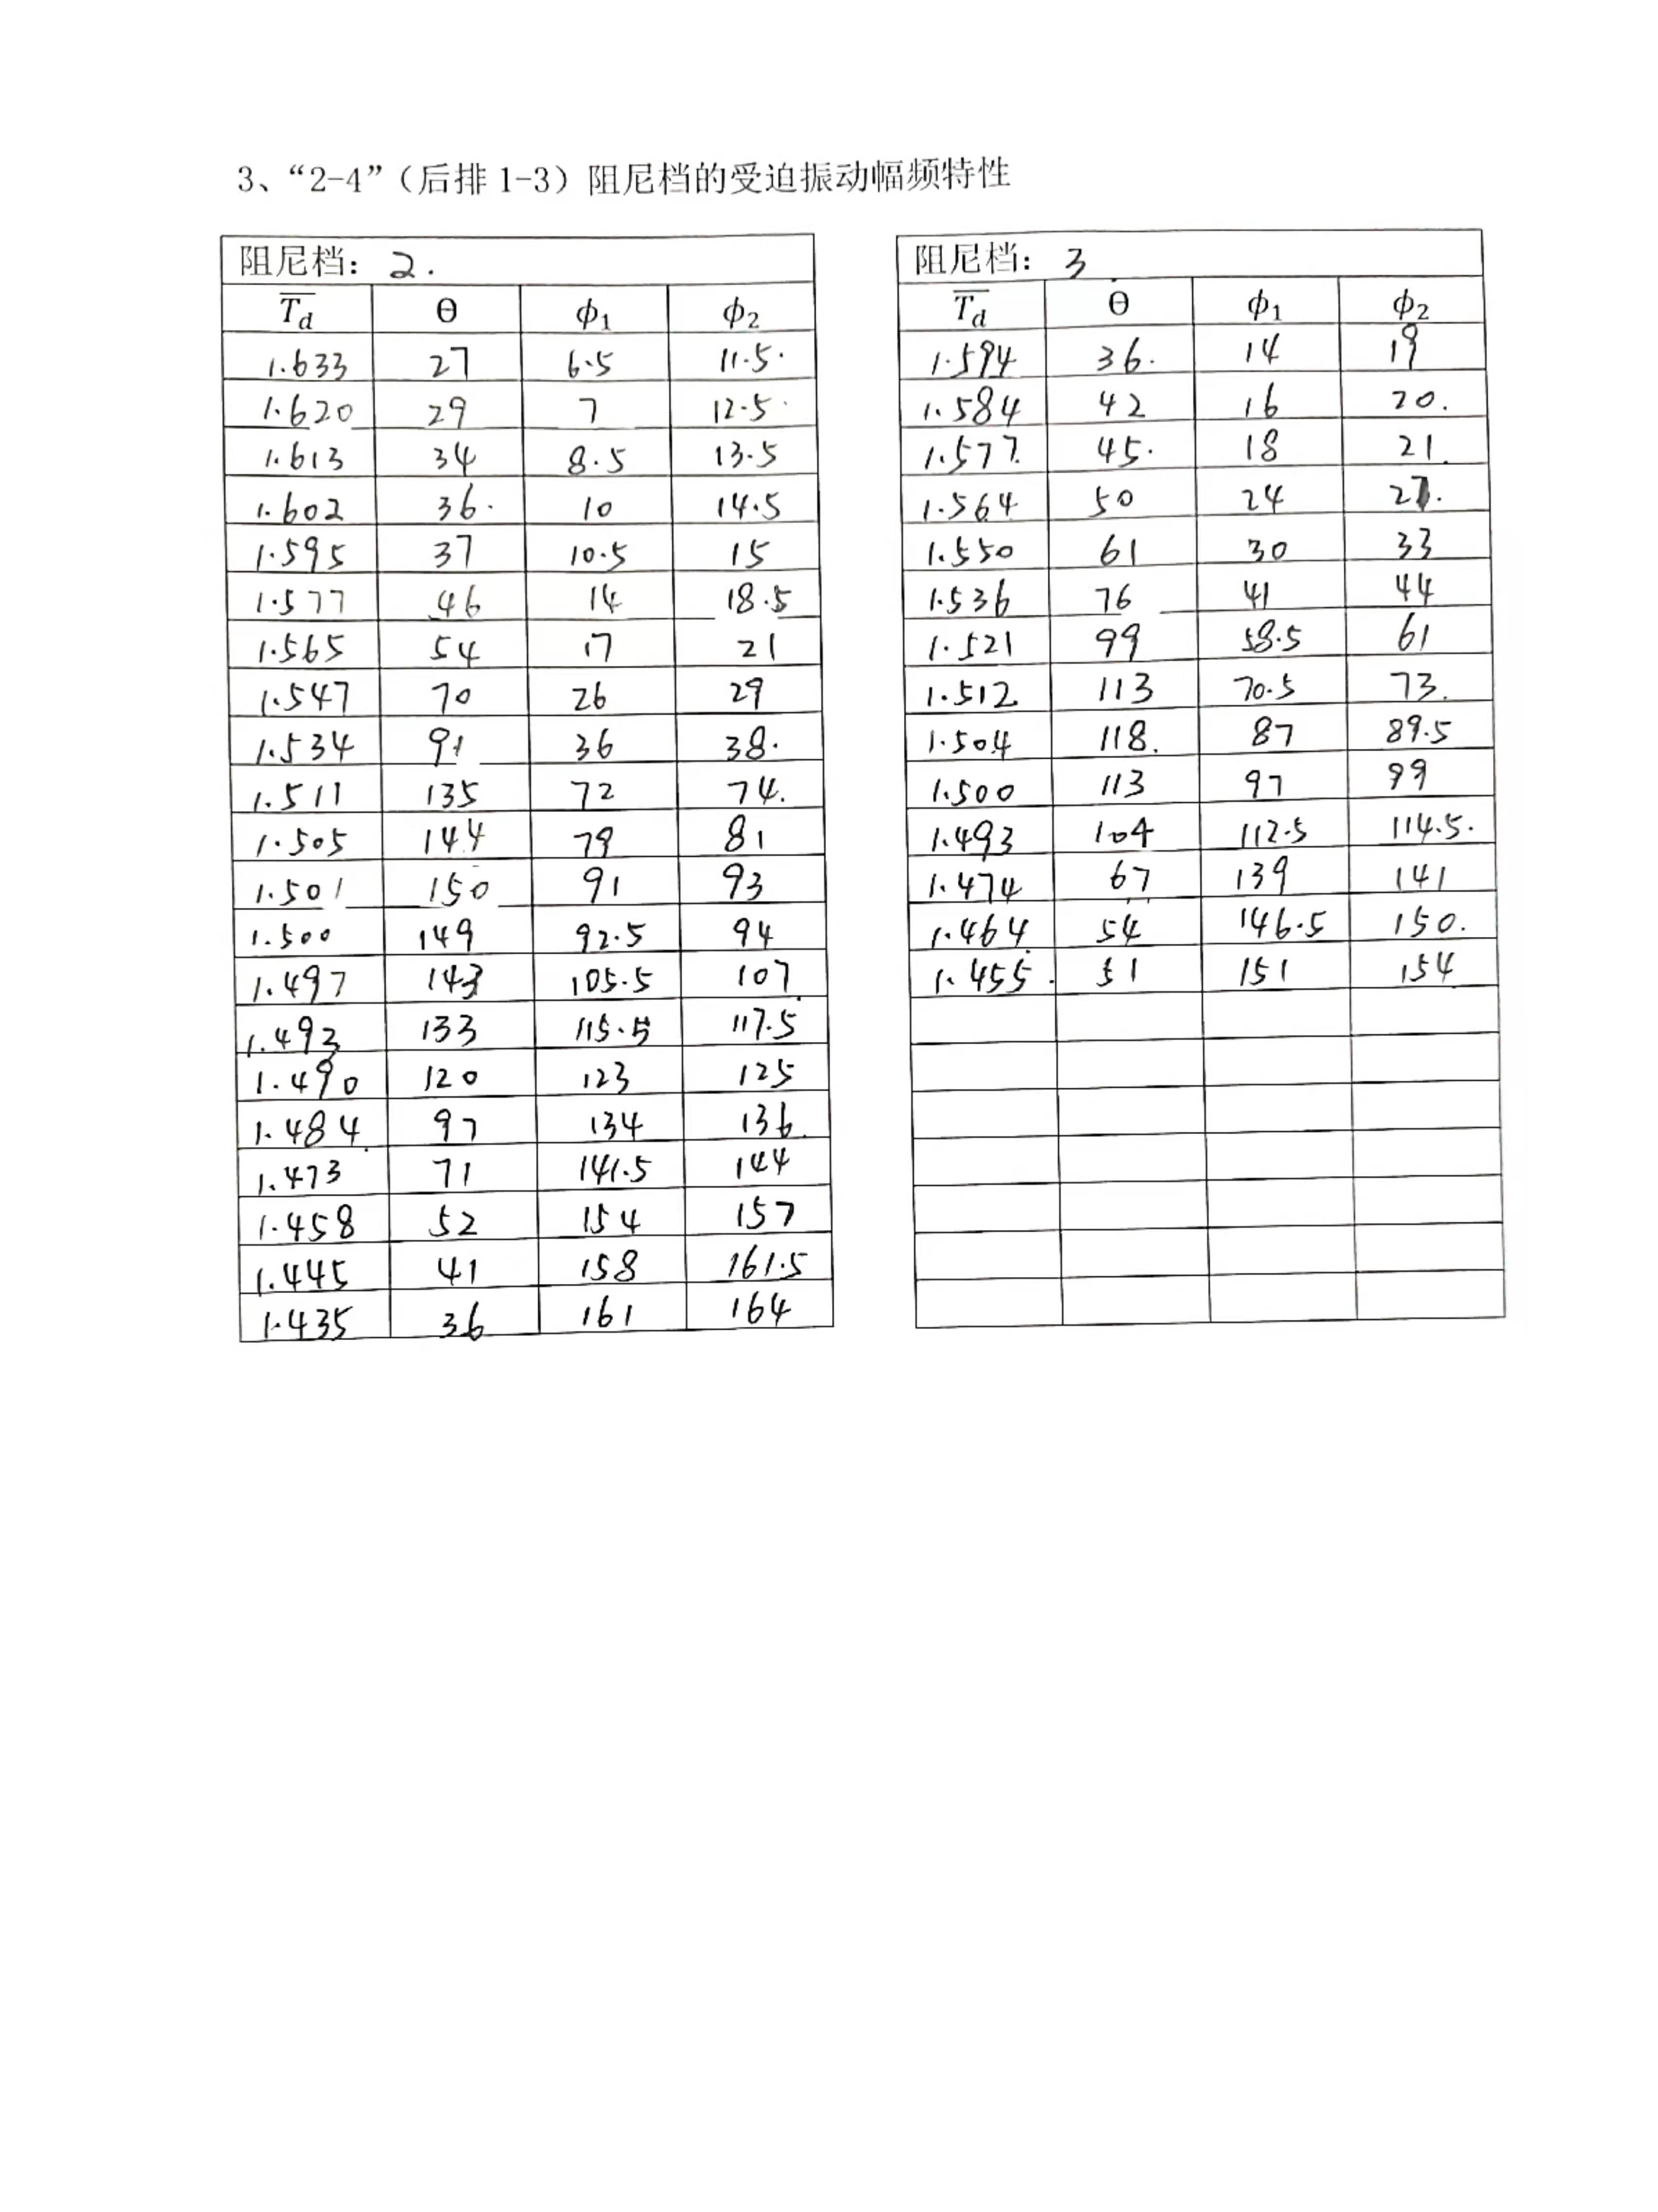
\includegraphics[scale=0.15]{原始数据2.jpg}
\end{figure}
\begin{figure}[H]
    \centering
    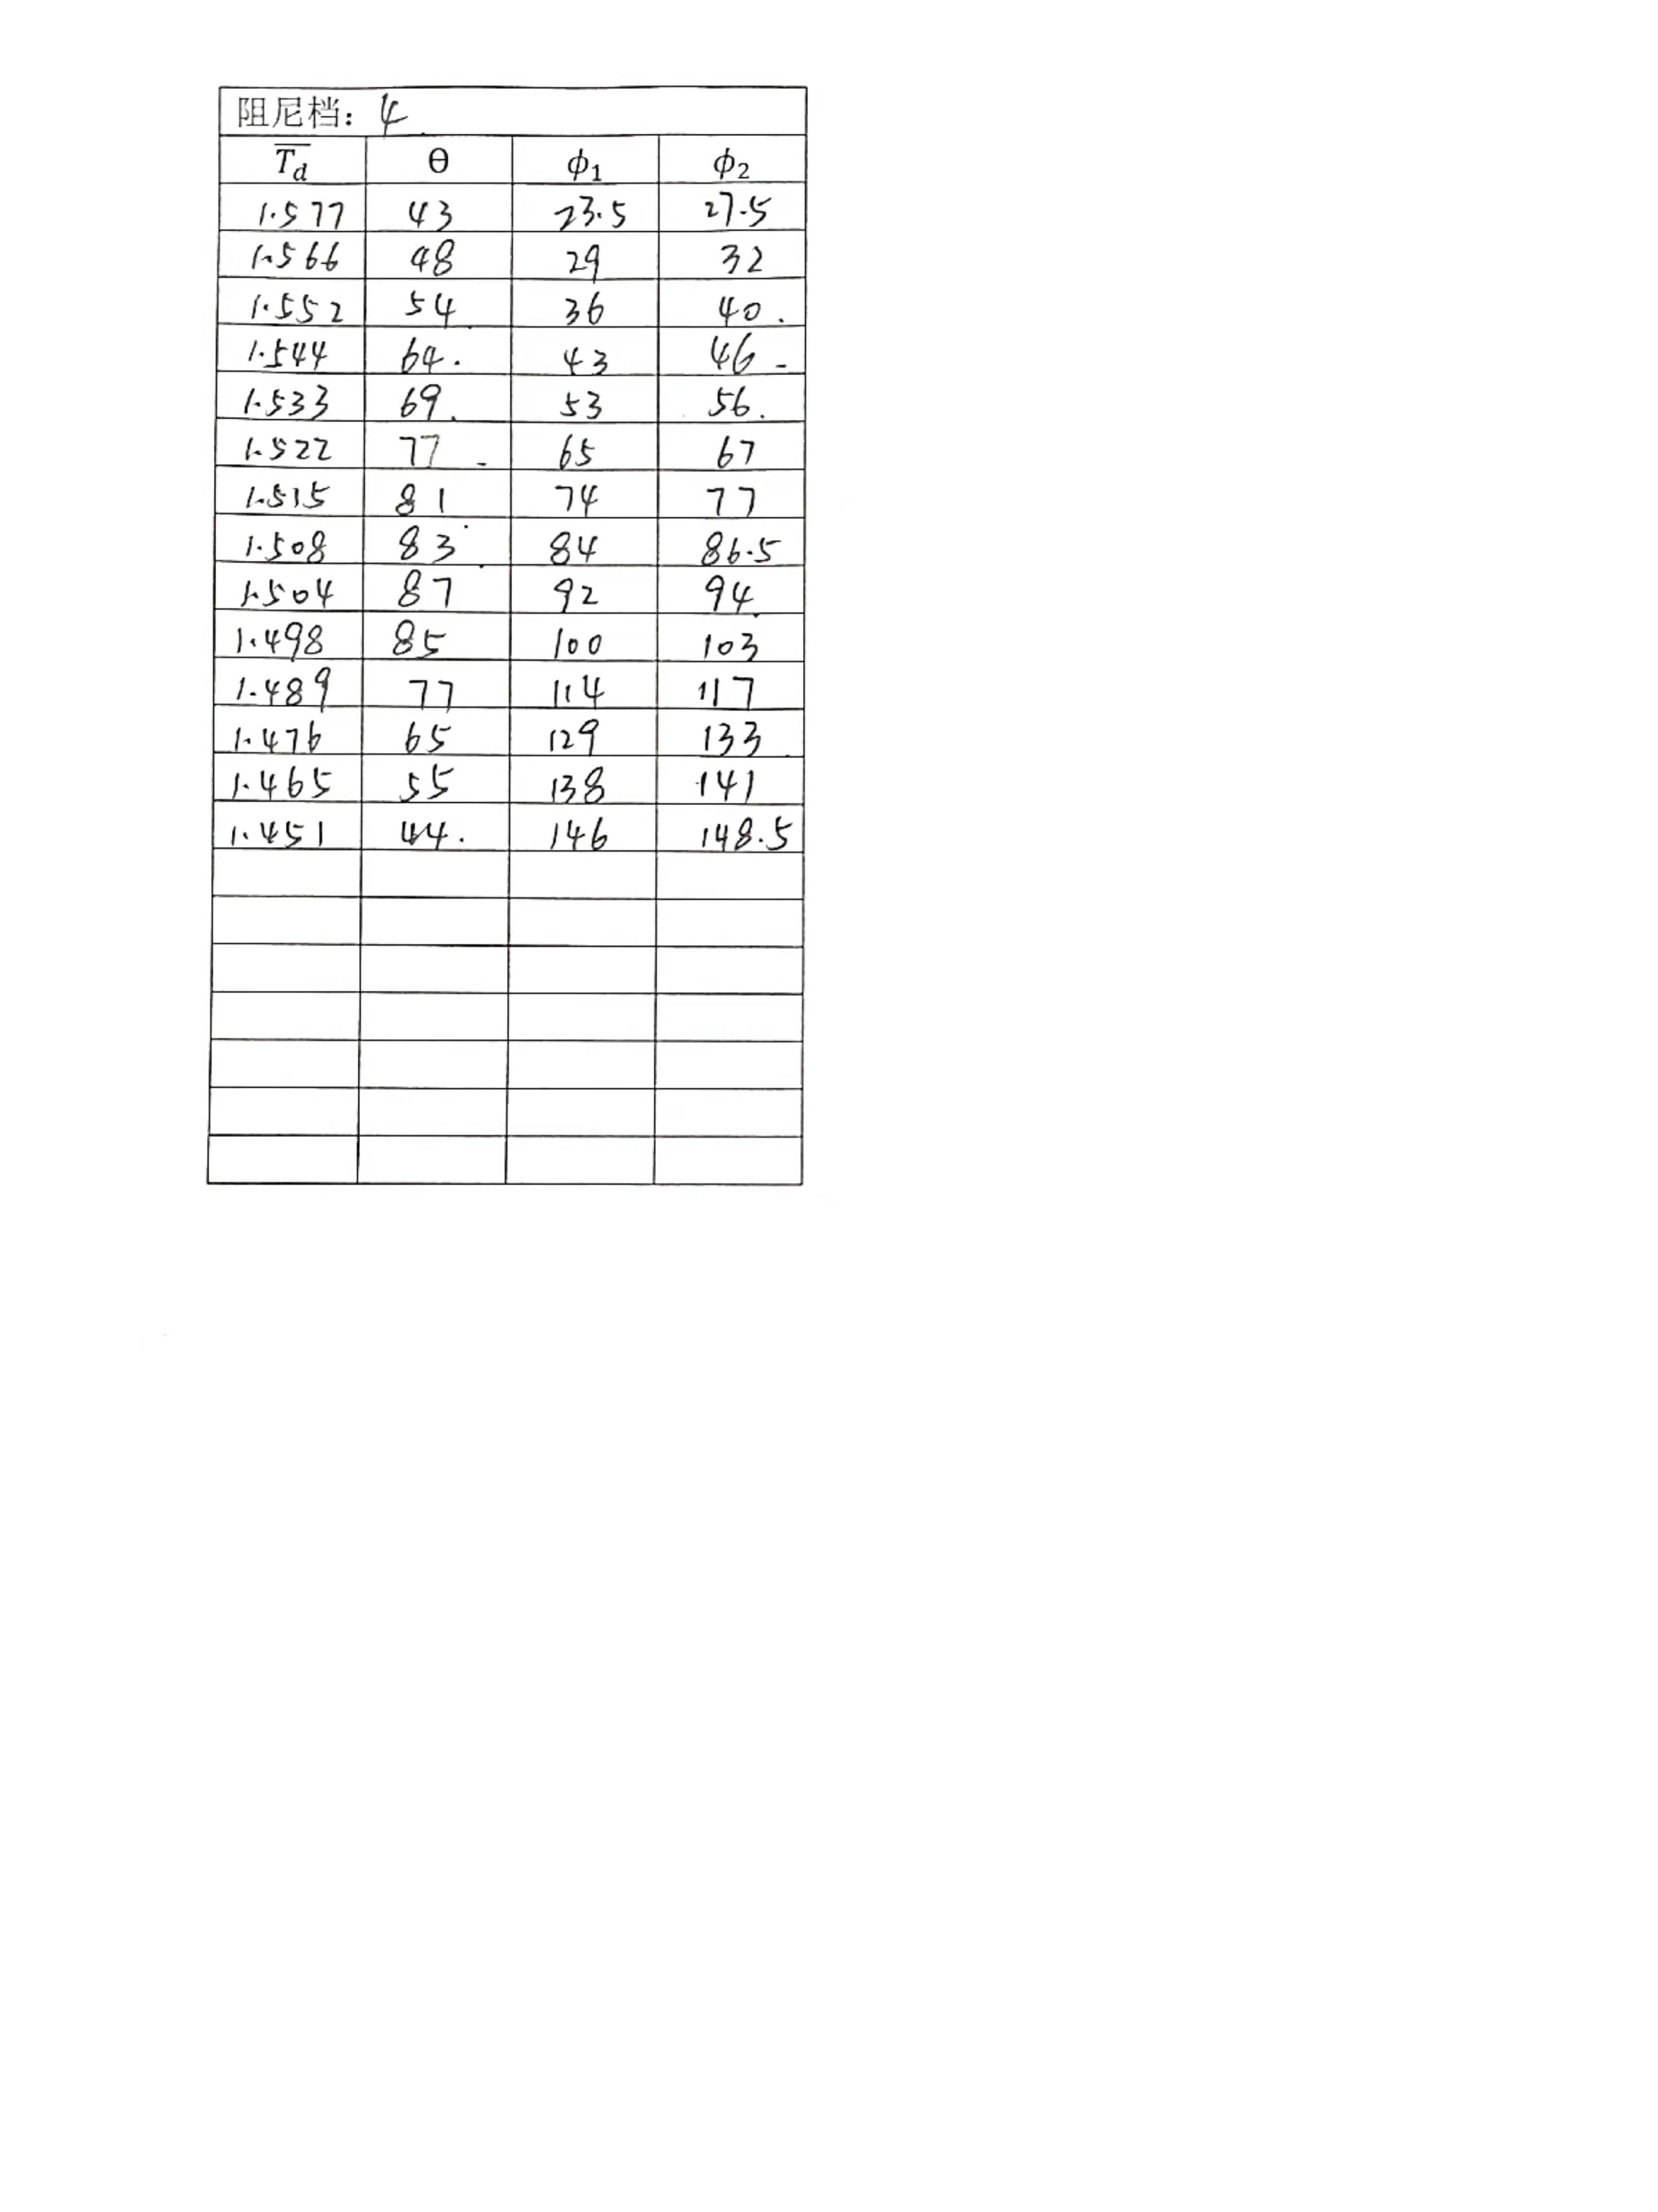
\includegraphics[scale=0.12]{原始数据3.jpg}

\end{figure}



\end{document}